\chapter{Overview}

In this chapter, we will provide a thorough overview of the project. We will begin by discussing the general context, covering both the educational and professional backgrounds. Next, we will detail the project itself, identifying the problem, reviewing existing solutions, and presenting our innovative approach. Lastly, we will describe the methodology used in the project, including the team structure and roles. This structured approach will ensure a comprehensive understanding of the project's scope, objectives, and implementation strategy.

\pagebreak

\section{General context}
This part is dedicated to present the project context such as the scholar and the professional frame.

\subsection{Pedagogical frame}

This project was undertaken as part of a graduation internship, the final step in obtaining an engineering degree in computer science from the Private Higher School of Engineering and Technology "ESPRIT" \hyperref[fig:ilef_logo]{(Logo: Figure \ref{fig:esprit_logo})}.
 The internship spanned six months, from January 1st to July 1st, 2024, during which I integrated with the development team at Ilef Export.
 

\begin{figure}[htbp]
  \centering  % Add this line to center the image
  \includegraphics[width=12cm]{./chapters/overview/esprit.jpeg}
  \caption{ESPRIT logo}
  \label{fig:esprit_logo}
\end{figure}

\subsection{Professional frame}
% \vspace*{64pt}

Ilef Export \hyperref[fig:ilef_logo]{(Logo: Figure \ref{fig:ilef_logo})} is a prominent Tunisian company headquartered in Tunisia. Specializing in the export of high-quality dates and vegetables, Ilef Export has established itself as a key player in the agricultural export industry. Founded with a commitment to excellence, the company has built a strong reputation for delivering premium products to its clients.

Ilef Export serves a range of distinguished clients, including Monoprix, and focuses its export efforts primarily on markets in Morocco, France, and Canada... The company's strategy is centered on maintaining stringent quality standards, ensuring exceptional customer satisfaction, and continuously expanding its market presence.
Through its dedication to quality and innovation, Ilef Export aims to solidify its position as a leader in the global agricultural export sector.

\begin{figure}[htbp]
  \centering  % Add this line to center the image
  \includegraphics[width=8cm]{./chapters/overview/ilef_logo.png}
  \caption{ILEF Export logo}
  \label{fig:ilef_logo}
\end{figure}



\section{Project presentation}
\subsection{Problematic}
Ilef Export, a leading exporter in Tunisia specializing in dates and vegetables, maintains a prominent presence in global markets such as Morocco, France, and Canada. However, the company faces several significant challenges in its cloud operations:

\begin{itemize}
  \item \textbf{Complex Management }:
  Managing services across multiple cloud providers (AWS, Google Cloud, Azure, and Hetzner) is complicated due to different tools and processes. This complexity leads to inefficiencies and increased operational costs.

  \item \textbf{Vendor Lock-In }:
  Relying on a single cloud provider creates a risk of vendor lock-in, making it difficult to switch or balance workloads across providers. This dependency limits flexibility and can potentially increase costs.

  \item \textbf{Time Inefficiencies }:
  Setting up instances/clusters and deploying Docker containers across various cloud providers takes a significant amount of time, causing delays in deployment and impacting overall productivity.

  \item \textbf{Cost Control }:
  Tracking and managing costs across different cloud providers is challenging, leading to unpredictable expenses and budget issues.

  \item \textbf{Lack of Unified Management }:
  Without a single platform to manage all cloud services efficiently, the teams face fragmented processes and poor resource utilization.
\end{itemize}


\subsection{Examination of current solutions}
To address the challenges in managing multi-cloud environments, it is crucial to examine existing solutions and their limitations. This evaluation will focus on three popular multi-cloud management platforms: \textbf{ Flexera} (formerly RightScale), \textbf{CloudBolt}, and \textbf{CloudHealth}.
\subsubsection{Flexera}
\begin{itemize}
  \begin{figure}[htbp]
    \centering  % Add this line to center the image
    \includegraphics[width=5cm]{./chapters/overview/flexera.jpg}
    \caption{Flexera logo}
    \label{fig:flexera}
  \end{figure}
  \item \textbf{Capabilities }:
Flexera provides a unified interface for managing multiple cloud environments, including AWS, Google Cloud. It offers features for cloud cost management, automated workflows, and governance.

\item \textbf{Limitations }:
\begin{negitemize}
  \item \textbf{Cost }: Flexera can be expensive, particularly for small to medium-sized enterprises. The pricing model can become a significant burden as the scale of cloud operations increases.
  \item \textbf{Complexity }: The initial setup and configuration of Flexera can be complex and time-consuming, requiring specialized knowledge and resources.
\end{negitemize}
\end{itemize}


\subsubsection{CloudBolt}

\begin{figure}[htbp]
  \centering  % Add this line to center the image
  \includegraphics[width=4cm]{./chapters/overview/cloudbolt.jpg}
  \caption{Cloudbolt logo}
  \label{fig:cloudbolt}
\end{figure}

\begin{itemize}
  \item \textbf{Capabilities }:
  CloudBolt offers comprehensive multi-cloud management, including provisioning, orchestration, and cost optimization. 
\item \textbf{Limitations }:
\begin{negitemize}
  \item \textbf{User Experience }: The user interface can be less intuitive compared to other platforms, leading to a steeper learning curve for new users.
  \item \textbf{Performance }: Some users have reported performance issues when managing large-scale deployments, which can impact overall efficiency.
\end{negitemize}
\end{itemize}

\subsubsection{CloudHealth}
\begin{figure}[htbp]
  \centering  % Add this line to center the image
  \includegraphics[width=6cm]{./chapters/overview/cloudhealth.png}
  \caption{Cloudhealth logo}
  \label{fig:cloudhealth}
\end{figure}

\begin{itemize}
  \item \textbf{Capabilities }:
  CloudHealth by VMware provides robust cloud cost management, governance, and security features across multiple cloud environments, including AWS, Google Cloud, and Azure.

\item \textbf{Limitations }:
\begin{negitemize}
  \item \textbf{Cost}:  CloudHealth can be relatively expensive, especially for smaller organizations. The pricing structure may become burdensome as cloud usage scales.
  \item \textbf{Provider Support }: CloudHealth does not support many cloud providers such as Hetzner, limiting its usefulness for organizations utilizing this provider.

\end{negitemize}
\end{itemize}

\subsection{The proposed solution}
To address the identified challenges and limitations of existing solutions, Ilef Export proposes the development of a unified platform tailored to its specific needs. This platform will streamline operations, enhance flexibility, and provide better visibility into costs across multiple cloud providers, including AWS, Google Cloud, Azure, and Hetzner.

The proposed solution includes the following key components:
\begin{positemize}
  \item \textbf{ Unified Interface:}
  Develop a single interface to manage virtual machines, containers, and other resources across all supported cloud providers.

  \item \textbf{ Automated Workflows:}
  Develop automated workflows for deploying Docker containers and setting up instances, significantly reducing the time and effort required for these processes.

  \item \textbf{ Cost Visualization: }
  Implement tools to track and visualize cloud costs, providing clear insights into expenses across different providers.

  \item \textbf{ Kubernetes Integration:}
  Include tools for managing Kubernetes clusters, simplifying the deployment and scaling of containerized applications to meet the company's specific needs.
\end{positemize}



\section{Methodology}
The software development process involves a series of tasks that result in the creation of new software or modifications to existing systems. No single process is flawless, and companies often adapt their methodologies based on specific needs, which can vary depending on stakeholders, circumstances, and project characteristics. The primary goal of a development methodology is to enhance the quality of the product. Adopting a project management methodology is crucial for helping team members achieve their goals within set time frames. 
\subsection{Agile Methodologies}
Agile methodology is a project management strategy commonly used in software development. This approach helps teams address the unpredictability of software creation through incremental, iterative work cycles known as sprints. A sprint is a designated time frame for completing a specific phase of a project. Once this period concludes, the sprint is considered finished, regardless of whether all team members agree on the development’s quality. The project continues to evolve in subsequent phases, each adhering to its scheduled duration. Agile emphasizes flexibility, continuous improvement, and collaboration, enabling teams to adapt to changes quickly and deliver high-quality software.
\subsection{Scrum method}
Scrum as shown in the \hyperref[fig:scrum]{(Figure \ref{fig:scrum})} is an iterative and incremental approach within agile software development. In Scrum, the sprint serves as the fundamental development unit. Each sprint begins with a planning session to outline tasks and set goals. At the end of the sprint, a review or retrospective meeting evaluates the progress and identifies lessons for future sprints. Throughout each sprint, the team works on producing completed segments of the product. Scrum promotes transparency, inspection, and adaptation, ensuring that the development process remains efficient and aligned with project goals. The key roles in Scrum include the Product Owner, Scrum Master, and Development Team, each contributing to the successful execution of sprints and overall project delivery.
\vspace{1cm}

Given the iterative changes and evolving requirements of our project, we have chosen the Agile methodology and the Scrum framework to ensure flexibility and continuous improvement.

\vspace{1cm}
\begin{figure}[htbp]
  \centering  % Add this line to center the image
  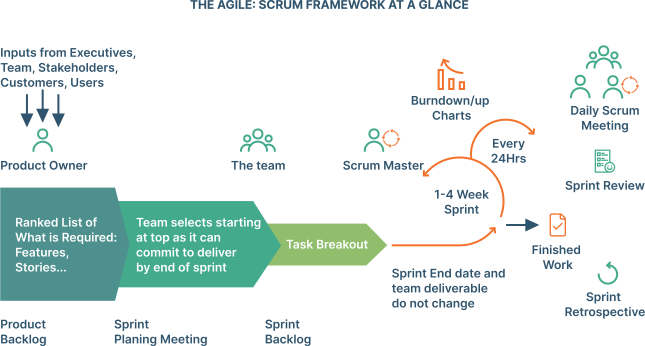
\includegraphics[width=13cm]{./chapters/overview/scrum.png}
  \caption{Scrum process}
  \label{fig:scrum}
\end{figure}

\vspace{1cm}
\subsubsection{Project team}
The table \hyperref[p]{\ref{p}} introduces the project team members and their roles.

\begin{table}[!htbp]
\centering
  \begin{tabular}{ | p{3cm}  | p{6cm} |}
    \hline

    Scrum role    & Name          \\ \hline

    Product owner & Abdelhamid Jemaa  \\ \hline
    Scrum Master  & Chaker Benhamad   \\ \hline
    Team members  & Mehrez Benhamad \\ \hline

    \hline
  \end{tabular}
\caption{Project members and roles}
\label{p}
\end{table}

\section*{Conclusion}
In this chapter, we have offered a detailed overview of the project, beginning with the general context that includes both pedagogical and professional frameworks. We identified the problem, evaluated existing solutions, and presented our innovative approach. Additionally, we outlined the project methodology, including the team composition and their roles. This structured approach has provided a clear understanding of the project's scope, objectives, and execution strategy.

By establishing this solid foundation, we are well-prepared for the subsequent phases of the project, enabling us to achieve our desired outcomes efficiently and effectively.

In the next chapter, "Preliminary Study," we will delve deeper into the initial research and analysis conducted to inform our project's direction.